\chapter{Centre Management}
\label{chap:centre-management}

A \entitytarget{Centre} can be one or a combination of the following:
\begin{description}

\item[Collection Centre] \hfill \\ Where specimens are collected from patients
  (e.g. a clinic).

\item[Processing Centre] \hfill \\ Where collected specimens are processed.

\item[Storage Centre] \hfill \\ Where collected and processed specimens are
  stored. Usually, a storage centre is also a processing centre.

\item[Request Centre] \hfill \\ Where collected and processed specimens are
  sent for analysis. Usually the specimens are stored first at a storage
  centre.
\end{description}

Figure \ref{fig:centre-aggregate} shows the \entitylink{Centre} aggregate. Its
attributes are: a short identifying name; a description that provides more
details on the name; and the \compfont{enabled} flag. When a centre is enalbed
it is ready to accept specimens. When disabled it is either being configured or
no longer in use.

\begin{figure}[H]
  \centering
  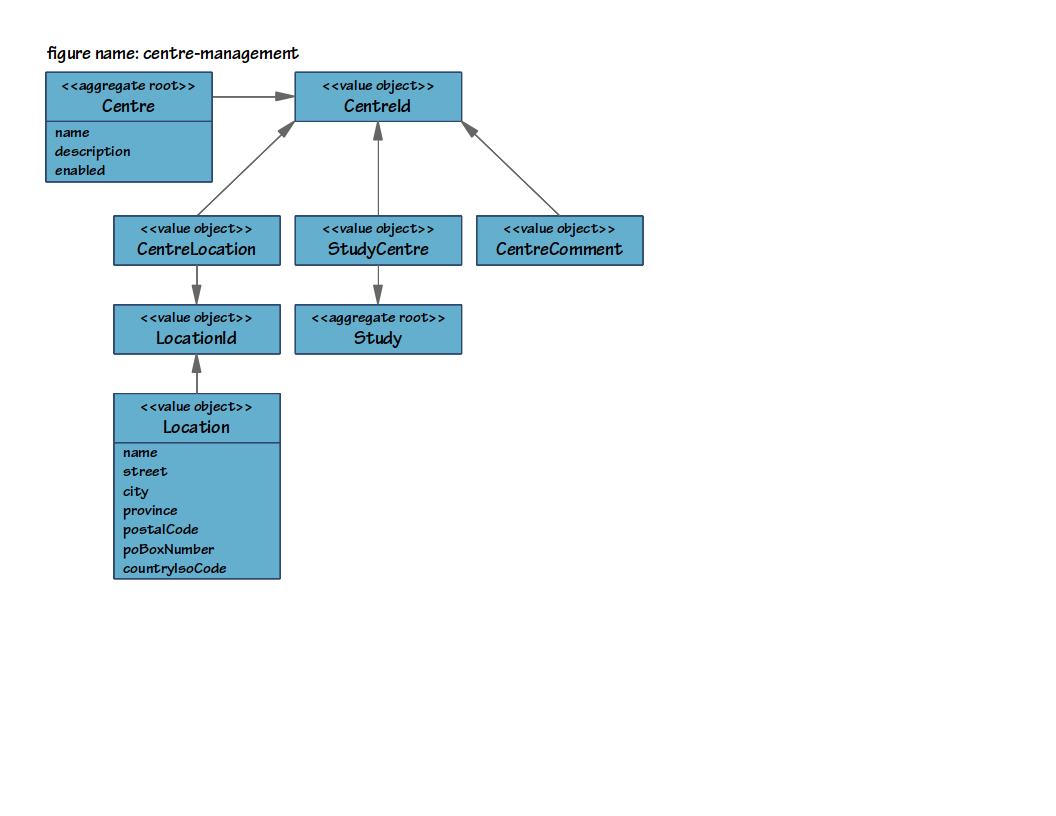
\includegraphics[trim={10mm 62mm 108mm 18mm}, clip,
    width=0.65\textwidth]{images/centre-management}
  \caption{Centre Aggregate}
  \label{fig:centre-aggregate}
\end{figure}

The model objects associated with a centre are described below.

\subsection*{CentreLocation}
A centre may have more than one location. \entitytarget{CentreLocation} is used
to record the locations.

\subsection*{Location}
A \entitytarget{Location} is a centre's street address. It has the usual
attributes for an address.

\subsection*{StudyCentre}
\entitylink{StudyCentre} is used to link a centre

\subsection*{CentreComment}
A \entitytarget{CentreComment} contains a textual message and the
user that added the comment. The date and time the comment was made is recorded
as meta data. A processing event can have one or more comments.

% Local Variables:
% compile-command: "/usr/bin/rubber --pdf main"
% End:
